\section{The pre-registered prompt study}
\label{app:grid}

This appendix reports the pre-registered prompt study: three models under five prompt conditions on the
grid, with its prompt checks, its zero-noise run and its independent check. It is the evidence behind
the over-confirmation in Section~\ref{sec:both}. Table~\ref{tab:cells} compares each cell with the guessing rule on
how good the best candidate it tested was and on how well it picked among what it tested.

\subsection{Setup}
\label{sec:envgrid}
\label{sec:design}

The grid uses the generated landscape, campaign, noise and failures of Section~\ref{sec:env} and
Appendix~\ref{app:env}. The agent is told only that it is running a numerical optimisation campaign, and never that
it is working on proteins.

\paragraph{Why the landscape is generated.} A generated landscape makes the true value of every candidate
known, and no model can have seen its best candidate. A published landscape cannot guarantee either. Given the GB1
protein landscape of \citet{wu2016adaptation} with its real amino-acid letters, Opus 4.7 named the best
measured variant in round one in 11 of 20 campaigns. Four random viable picks would do so 0.035\% of the
time. The prompt study uses the grid only, and the five-model study adds GB1 and PhoQ.

\paragraph{Five prompt conditions.} Five conditions vary what the agent is told, each adding to the one
before. \textbf{Blind} says nothing about measurement error. \textbf{Quantitative} adds that readings carry
error and gives $\sigma(f)$. \textbf{Mechanism} adds that averaging $n$ readings reduces the standard error
by $\sqrt{n}$, and permits re-ordering, without recommending it. \textbf{Aggregated} keeps Mechanism's text
and changes the environment: the history is shown as a count, mean and standard error per
candidate, in place of one line per reading. \textbf{Decision-rule} adds the selection rule outright. No
condition ever instructs the agent to re-test, because that would measure instruction-following.

\begin{sloppypar}
\paragraph{Models and scale.} Three models, called Opus 4.7, Gemini 2.5 Flash and DeepSeek V3.1
throughout this paper and requested from OpenRouter as \texttt{anthropic/claude-opus-4.7},
\texttt{google/gemini-2.5-flash} and \texttt{deepseek/deepseek-chat-v3.1}, at temperature 0. We call one
model under one prompt condition a \emph{cell}, so the prompt study has 15 cells. It holds
5{,}075 campaigns and 162{,}986 model calls. Cells are sized per model, so $N$ is 695, 139 and 181
campaigns per cell respectively.
\end{sloppypar}

\paragraph{Pre-registration.} The design, the outcome, the six confirmatory contrasts and the analysis were
fixed before the prompt study ran (Appendix~\ref{app:amendments}). The six contrasts are Aggregated against Mechanism and
Decision-rule against Mechanism, for each model, with Holm correction for multiple comparisons across the six.
Contrasts are paired by seed. The seed fixes measurement noise and failures, so at a given seed the $k$-th reading
of a candidate is the same in every condition.

\paragraph{The scripted rules.} The guessing and informed rules of Appendix~\ref{app:refs} are the grid's
references. Both do best at $k^\ast = 1$, one slot in four.

\subsection{Results}
\label{sec:results}

\begin{figure}[tbp]
\centering
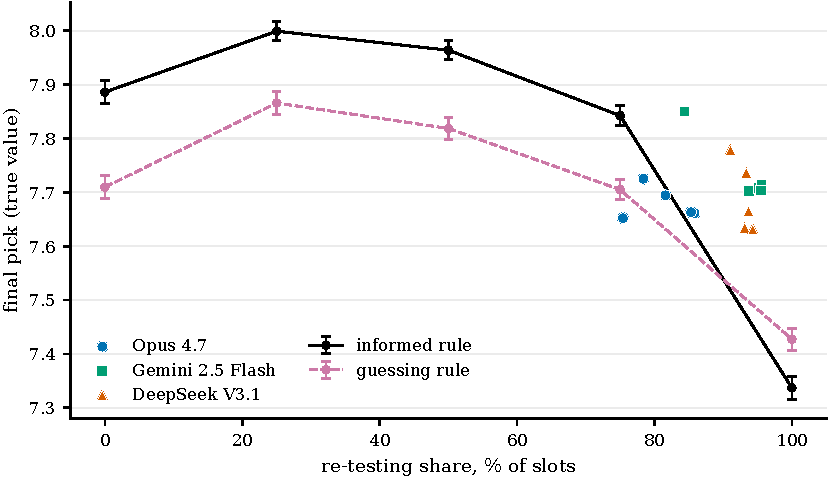
\includegraphics[width=\textwidth]{fig2_outcome_vs_replication.pdf}
\caption{True value of the final pick against the re-testing share, one point per cell. The two lines are the
informed rule (upper, told which candidates are viable) and the guessing rule (lower), spending $k=0$ to 4 of the
four slots each round re-testing their current best, with 95\% intervals.}
\label{fig:gridheadline}
\end{figure}

\subsubsection{Re-testing share}

Agents spend most of their measurements re-testing candidates they have already measured. Across the 15
cells the re-testing share runs from 75\% to 96\% of used slots; both scripted rules spend a
quarter (Table~\ref{tab:cells}, Figure~\ref{fig:gridheadline}). The count includes re-orders of the reference
candidate, whose score the agent is given at the start. On this count every cell re-tests more than a
scripted protocol that measures each candidate three times (Appendix~\ref{app:further}). Without those re-orders the share is 57\% to
75\%, and six cells fall below that protocol. Counting only slots spent on a candidate that already has a successful
reading, which leaves out re-orders after a failed order, gives 74.7\% to 95.1\%, within 1.4 points of the headline
in every cell.

% Generated by scripts/make_table_cells.py from results/analysis_final/grid/summary.json.
% Do not edit by hand; verify_paper_numbers.py regenerates it and fails on any difference.
\begin{table}[tbp]
\centering
\small
\caption{Results for each cell, one model under one prompt condition. \emph{Share} is the re-testing share, the fraction of used slots spent re-testing a candidate already ordered. \emph{Excl.\ start} leaves out re-orders of the start, whose reading the agent is given in advance. \emph{Distinct} is the mean number of different candidates measured per campaign, and \emph{pick} the mean true value of the final pick. The last three columns compare each cell with the guessing rule at its best setting, which measures 28.94 distinct candidates and reaches 7.87. \emph{Tested} is how much further the best candidate the agents measured falls short of the global best. \emph{Picked} is the change in how far their pick falls short of the best they measured, negative where they picked better. \emph{Net} is the sum, the agents' shortfall in the true value of the final pick; rounded parts may not add to it exactly.}
\label{tab:cells}
\begin{tabular}{llrrrrrrr}
\toprule
 & & \multicolumn{2}{c}{share (\%)} & & & \multicolumn{3}{c}{against the guessing rule} \\
\cmidrule(lr){3-4}\cmidrule(lr){7-9}
model & condition & all & excl.\ start & distinct & pick & tested & picked & net \\
\midrule
Opus 4.7 & Blind & 75.4 & 62.8 & 11.3 & 7.65 & $+0.33$ & $-0.12$ & $+0.21$ \\
 & Quantitative & 78.4 & 65.5 & 10.4 & 7.73 & $+0.25$ & $-0.11$ & $+0.14$ \\
 & Mechanism & 81.6 & 68.1 & 9.0 & 7.69 & $+0.31$ & $-0.14$ & $+0.17$ \\
 & Aggregated & 85.8 & 70.4 & 7.0 & 7.66 & $+0.37$ & $-0.17$ & $+0.20$ \\
 & Decision-rule & 85.3 & 70.8 & 7.3 & 7.66 & $+0.36$ & $-0.16$ & $+0.20$ \\
\addlinespace
Gemini 2.5 Flash & Blind & 93.8 & 69.5 & 3.3 & 7.70 & $+0.37$ & $-0.21$ & $+0.16$ \\
 & Quantitative & 84.4 & 67.3 & 7.7 & 7.85 & $+0.18$ & $-0.16$ & $+0.02$ \\
 & Mechanism & 95.2 & 73.3 & 2.7 & 7.71 & $+0.38$ & $-0.22$ & $+0.16$ \\
 & Aggregated & 95.6 & 74.6 & 2.6 & 7.71 & $+0.37$ & $-0.22$ & $+0.15$ \\
 & Decision-rule & 95.5 & 73.8 & 2.6 & 7.70 & $+0.38$ & $-0.21$ & $+0.16$ \\
\addlinespace
DeepSeek V3.1 & Blind & 91.0 & 68.6 & 4.9 & 7.78 & $+0.26$ & $-0.17$ & $+0.09$ \\
 & Quantitative & 93.1 & 63.1 & 3.9 & 7.63 & $+0.41$ & $-0.18$ & $+0.23$ \\
 & Mechanism & 93.7 & 56.9 & 3.7 & 7.66 & $+0.38$ & $-0.18$ & $+0.20$ \\
 & Aggregated & 94.3 & 57.0 & 3.4 & 7.63 & $+0.43$ & $-0.19$ & $+0.24$ \\
 & Decision-rule & 93.4 & 58.8 & 3.8 & 7.74 & $+0.31$ & $-0.18$ & $+0.13$ \\
\bottomrule
\end{tabular}
\end{table}


Re-testing buys something. Agents picked well among the candidates they had measured, closer to the best of
what they tested than the guessing rule. The best candidate they tested was much worse than that rule's best, because they tested so few (Figure~\ref{fig:gridsplit}). In every cell the shortfall from testing too few outweighs
the gain from picking well, so the agents end up behind (Table~\ref{tab:cells}, Figure~\ref{fig:shortfall_global}).
Their stated reasons show that they climb from their current best one letter at a time, as the scripted rules do,
in lines such as \emph{``vary pos4, C works
so try neighbor''}. They climb a few steps and then spend most of the budget confirming the same few candidates, so
the climb stalls.
 

\begin{figure}[tbp]
\centering
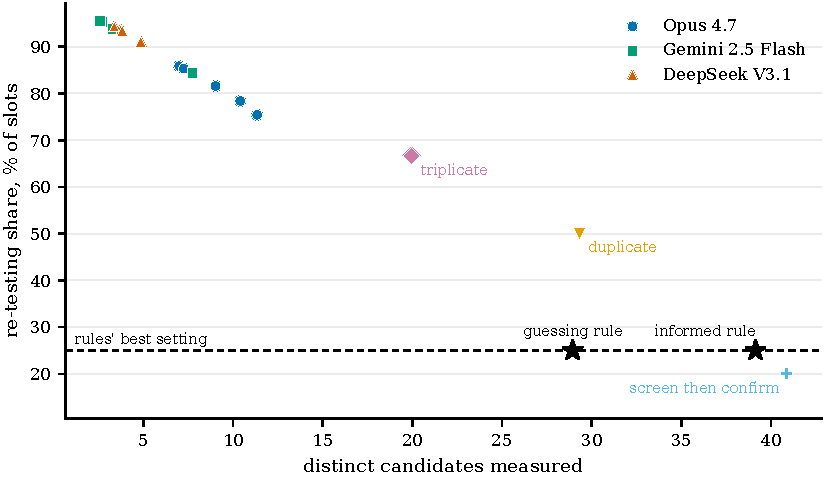
\includegraphics[width=\textwidth]{fig3_replication_vs_exploration.pdf}
\caption{Re-testing share against distinct candidates measured, one point per cell, with the informed and
guessing rules at their best setting and the three scripted lab protocols of Appendix~\ref{app:further}.}
\label{fig:gridsplit}
\end{figure}


\subsubsection{Exact readings}

Removing the noise lowers re-testing in every cell, significantly in 12 of 15. Re-testing still takes roughly half
to nearly all of the slots, and with exact readings no re-test is needed. The zero-noise run sets $\sigma$ to zero and changes nothing
else, so the agent is not told its readings are exact; Section~\ref{sec:indep} tests the case where it is
told. Here re-testing is counted after the first repeat an agent sees, as the share of slots spent on a candidate
that already has a successful reading. This is a stricter count than the headline share, and it is compared with the
same count under noise at the same seeds (Figure~\ref{fig:zero}; Appendix~\ref{app:further} gives the ranges and
intervals).

\begin{figure}[tbp]
\centering
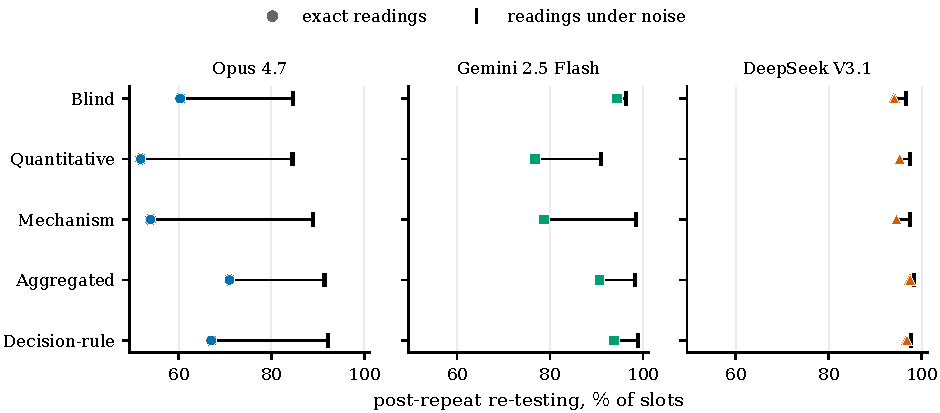
\includegraphics[width=\textwidth]{fig5_zero_noise.pdf}
\caption{Re-testing after the first repeat when every reading is exact (the marker) and the level implied under
noise (the bar), one row per cell. A repeat of an exactly known value returns no new information.}
\label{fig:zero}
\end{figure}

\subsubsection{Independent check}
\label{sec:indep}

In a separate one-round test with exact readings, the models still spent from about a quarter to over half
of the round re-testing. Saying the readings were exact made no detectable difference, and adding noise
raised re-testing sharply, so the models do respond to noise. The test was written separately from
Wellocate, with its own world generator, prompt and scorer, and shares no code with it. By a reading rule
fixed before any call, it confirms the behaviour in two of the three models and partly in Opus 4.7
(Appendix~\ref{app:indep}).

\subsubsection{Pre-registered contrasts}

If the behaviour came from a history that is hard to read, or from a missing rule, fixing those should reduce
it. Six contrasts were fixed before the prompt study ran, comparing Aggregated and Decision-rule with Mechanism for
each model, with Holm correction across the six (Table~\ref{tab:confirm}). One survives the correction: giving the selection rule outright improved the final pick for DeepSeek V3.1,
by $+0.0699$. It did not hold up: a pre-registered replication on 120 new seeds gave $+0.008$
$[-0.036, +0.052]$ (Appendix~\ref{app:replication}). In the original run the gain came through what DeepSeek V3.1 measured. Against the guessing rule, its
shortfall in the best candidate tested fell from 0.38 to 0.31, and its selection gain stayed at 0.18: it picked
among what it tested as well as before (Table~\ref{tab:cells}). It
picked the highest-average candidate about as often with the rule as without it (86\% against 90\%; an exact
McNemar test for paired choices gives $p = 0.36$). Its re-testing share moved by less than half a point (93.7\% against 93.4\%), and it tried
about as many candidates (3.7 against 3.8). Opus 4.7 responded differently. The rule raised its
highest-average picks from 74\% to 86\% ($p < 0.001$), and it also re-tested more and tried about two fewer
candidates. Opus 4.7 was nominally worse under both interventions; its unadjusted intervals exclude zero, and both differences lose significance after correction for the six contrasts. Gemini 2.5 Flash showed no detectable change.
Arithmetic alone does not explain the habit either: the Aggregated condition shows each candidate's count, mean and
standard error already computed, and re-testing was slightly higher under it than under Mechanism for all three
models. We do not read any of this as evidence that stating a decision rule helps agents.

\begin{table}[tbp]
\centering
\small
\caption{The six confirmatory contrasts on the final pick's true value, paired by seed, with Holm correction
across the family. The primary $p$ comes from a bootstrap that resamples seeds (studentised wild cluster bootstrap, 20{,}000 draws). The intervals are unadjusted and the Holm $p$ adjusts for the family of six. Seed
counts differ because each model's cells were sized separately (Section~\ref{sec:design}). $^\dagger$Did not hold up on 120 new seeds: $+0.008$, 95\% bootstrap interval $[-0.036, +0.052]$
(Appendix~\ref{app:replication}).}
\label{tab:confirm}
\begin{tabular}{llrrrr}
\toprule
model & contrast & seeds & diff & 95\% CI & Holm $p$ \\
\midrule
Opus 4.7     & Aggregated    & 695 & $-0.0334$ & $[-0.0606, -0.0061]$ & 0.0873 \\
Opus 4.7     & Decision-rule & 695 & $-0.0316$ & $[-0.0583, -0.0049]$ & 0.0873 \\
DeepSeek V3.1& Aggregated    & 181 & $-0.0332$ & $[-0.0757, +0.0092]$ & 0.3721 \\
DeepSeek V3.1& Decision-rule & 180 & $+0.0699$ & $[+0.0271, +0.1126]$ & \textbf{0.0075}$^\dagger$ \\
Gemini 2.5 Flash & Aggregated    & 139 & $+0.0067$ & $[-0.0130, +0.0265]$ & 1.0000 \\
Gemini 2.5 Flash & Decision-rule & 139 & $-0.0044$ & $[-0.0278, +0.0189]$ & 1.0000 \\
\bottomrule
\end{tabular}
\end{table}

\subsubsection{Prompt checks}
\label{sec:prompt}

A review of the prompts found two flaws. The round and replacement prompts did not say that the final pick is
scored on its true value. The replacement prompt also stated one order per round, where a round has four. A
wrong guess about viability could cost a slot, so rejection risk might also push agents toward re-testing
candidates known to work. We reran Blind and Mechanism for all three models on 60 seeds, each paired with the
original campaign on the same seed (Table~\ref{tab:prompt}, Appendix~\ref{app:prompt}). Prompt check A fixed the two flaws. In five of six cells the re-testing
share moved by less than 1.1 points. For Gemini 2.5 Flash under Blind it fell by 4.6 points [$-6.6$, $-2.6$],
and under Mechanism Gemini's final pick fell by 0.160 [$-0.256$, $-0.070$]. The registered margin for final picks,
$\pm 0.06$, could not be met with 60 pairs in four cells even with no true change. The re-testing share is
therefore the informative outcome. A rerun of the original prompts on the same day moved the re-testing share by at most 1.1 points from the original campaigns in every cell. The two Gemini shifts remain against this
control, so they come from the wording.

% Generated by scripts/make_table_prompt.py from results/analysis_0al.json.
% Do not edit by hand; verify_paper_numbers.py regenerates it and fails on any difference.
\begin{table}[tbp]
\centering
\small
\caption{Re-testing share in the prompt checks, as a percentage of used slots, on the same 60 seeds in every column. \emph{Grid} is the original campaigns on those seeds. Check~A states that the final pick is scored on its true value and corrects the replacement prompt's order count. Check~B also makes a rejected order free. \emph{Same-day rerun minus grid} is the change, in points, for the original prompts run again on the same day as check~A.}
\label{tab:prompt}
\begin{tabular}{llrrrr}
\toprule
model & condition & grid & check A & check B & same-day rerun minus grid \\
\midrule
Opus 4.7 & Blind & 76.0 & 76.6 & 74.8 & $-1.1$ \\
 & Mechanism & 82.1 & 81.1 & 80.9 & $+0.2$ \\
\addlinespace
Gemini 2.5 Flash & Blind & 94.4 & 89.8 & 83.3 & $-0.1$ \\
 & Mechanism & 95.2 & 95.1 & 89.0 & $-0.9$ \\
\addlinespace
DeepSeek V3.1 & Blind & 90.8 & 90.4 & 90.0 & $-0.9$ \\
 & Mechanism & 93.6 & 93.6 & 93.5 & $+0.1$ \\
\bottomrule
\end{tabular}
\end{table}


Prompt check B also made a rejected order free, so the agent simply chose again. Every cell still spent 74.8\% or more of its slots on re-tests, against 23.96\% for
the guessing rule at its best setting under the same rule. Gemini 2.5 Flash re-tested 6 to 11 points less and picked better, and it stayed far above the
guessing rule.
